% Created 2023-07-16 Sun 23:22
% Intended LaTeX compiler: xelatex
\documentclass[aspectratio=1610,xcolor={dvipsnames},hyperref={colorlinks,unicode,linkcolor=violet,anchorcolor=BlueViolet,citecolor=YellowOrange,filecolor=black,urlcolor=Aquamarine}]{beamer}
\usepackage{graphicx}
\usepackage{grffile}
\usepackage{longtable}
\usepackage{booktabs}
\usepackage{wrapfig}
\usepackage{rotating}
\usepackage[normalem]{ulem}
\usepackage{amsmath}
\usepackage{textcomp}
\usepackage{amssymb}
\usepackage{capt-of}
\usepackage{nicefrac}
\usepackage[dvipsnames]{xcolor}
\usepackage[colorlinks,unicode,linkcolor=violet,anchorcolor=BlueViolet,citecolor=YellowOrange,filecolor=black,urlcolor=Aquamarine]{hyperref}
\AtBeginSubsection[]{\begin{frame}<beamer>\frametitle{Section}\tableofcontents[currentsection,currentsubsection]\end{frame}}
\synctex=1
\usepackage{etoolbox}
\useoutertheme{infolines}
\setbeamertemplate{frametitle}{%
\usebeamerfont{frametitle}\insertframetitle\strut%
\vskip-0\baselineskip%
\leaders\vrule width .95\paperwidth\vskip1pt%
\vskip0pt%
\nointerlineskip%
}

%% T for footer
\setbeamercolor{footlinecolor}{fg=cyan,bg=green}
\setbeamercolor{author in head/foot}{fg=blue}
\setbeamertemplate{footline}{%
\leavevmode%
\hbox{%
\begin{beamercolorbox}[wd=.26\paperwidth,ht=2.25ex,dp=1ex,left]{author in head/foot}%
\hspace*{2ex}\usebeamerfont{author in head/foot} Dept. CSE, UT Arlington
\end{beamercolorbox}%
\begin{beamercolorbox}[wd=.50\paperwidth,ht=2.25ex,dp=1ex,center]{author in head/foot}%
\usebeamerfont{title in head/foot}Scalable Modeling \& Imaging \& Learning Lab (SMILE)
\end{beamercolorbox}%
\begin{beamercolorbox}[wd=.24\paperwidth,ht=2.25ex,dp=1ex,right]{date in head/foot}%
\usebeamerfont{date in head/foot}
\insertshortdate{}\hspace*{1em}  % date
\insertframenumber/\inserttotalframenumber\hspace*{2ex}
\end{beamercolorbox}}%
\vskip0pt%
}
\setbeamerfont{footnote}{size=\tiny}
\usepackage{minted}
\setbeamerfont{caption}{size=\scriptsize}
\usetheme{default}
\usefonttheme{serif}
\useinnertheme{circles}
\author{Nasy}
\date{Jul 16, 2023}
\title{Multimodal Large Language Model (MLLM)}
\hypersetup{
 pdfauthor={Nasy},
 pdftitle={Multimodal Large Language Model (MLLM)},
 pdfkeywords={},
 pdfsubject={},
 pdfcreator={Emacs 29.0.50 (Org mode 9.5.5)}, 
 pdflang={English}}
\usepackage{biblatex}
\addbibresource{/Users/Nasy/.emacs.d/萚兮/時/refs/ref.bib}
\begin{document}

\maketitle
\begin{frame}{Outline}
\setcounter{tocdepth}{1}
\tableofcontents
\end{frame}

\setcounter{tocdepth}{2}

\section{Introduction}
\label{sec:orgd4394ca}

\begin{frame}[label={sec:org8755cc1}]{Introduction}
\begin{itemize}
\item What is Multimodal Large Language Model (MLLM)?
\begin{itemize}
\item LLM-based model with the ability to receive and reason with multimodal information.
\end{itemize}
\item Future?
\begin{itemize}
\item MLLM is more in line with the way humans perceive the world.
\item MLLM offers a more user-friendly interface.
\end{itemize}
\item Examples
\begin{itemize}
\item GPT4
\item LLaVA
\item MiniGPT-4
\item \ldots{}
\end{itemize}
\end{itemize}
\end{frame}

\begin{frame}[label={sec:orga489961}]{Benchmark}
MME: A Comprehensive Evaluation Benchmark for Multimodal Large Language Models\footfullcite{fuMMEComprehensiveEvaluation2023}

\begin{center}
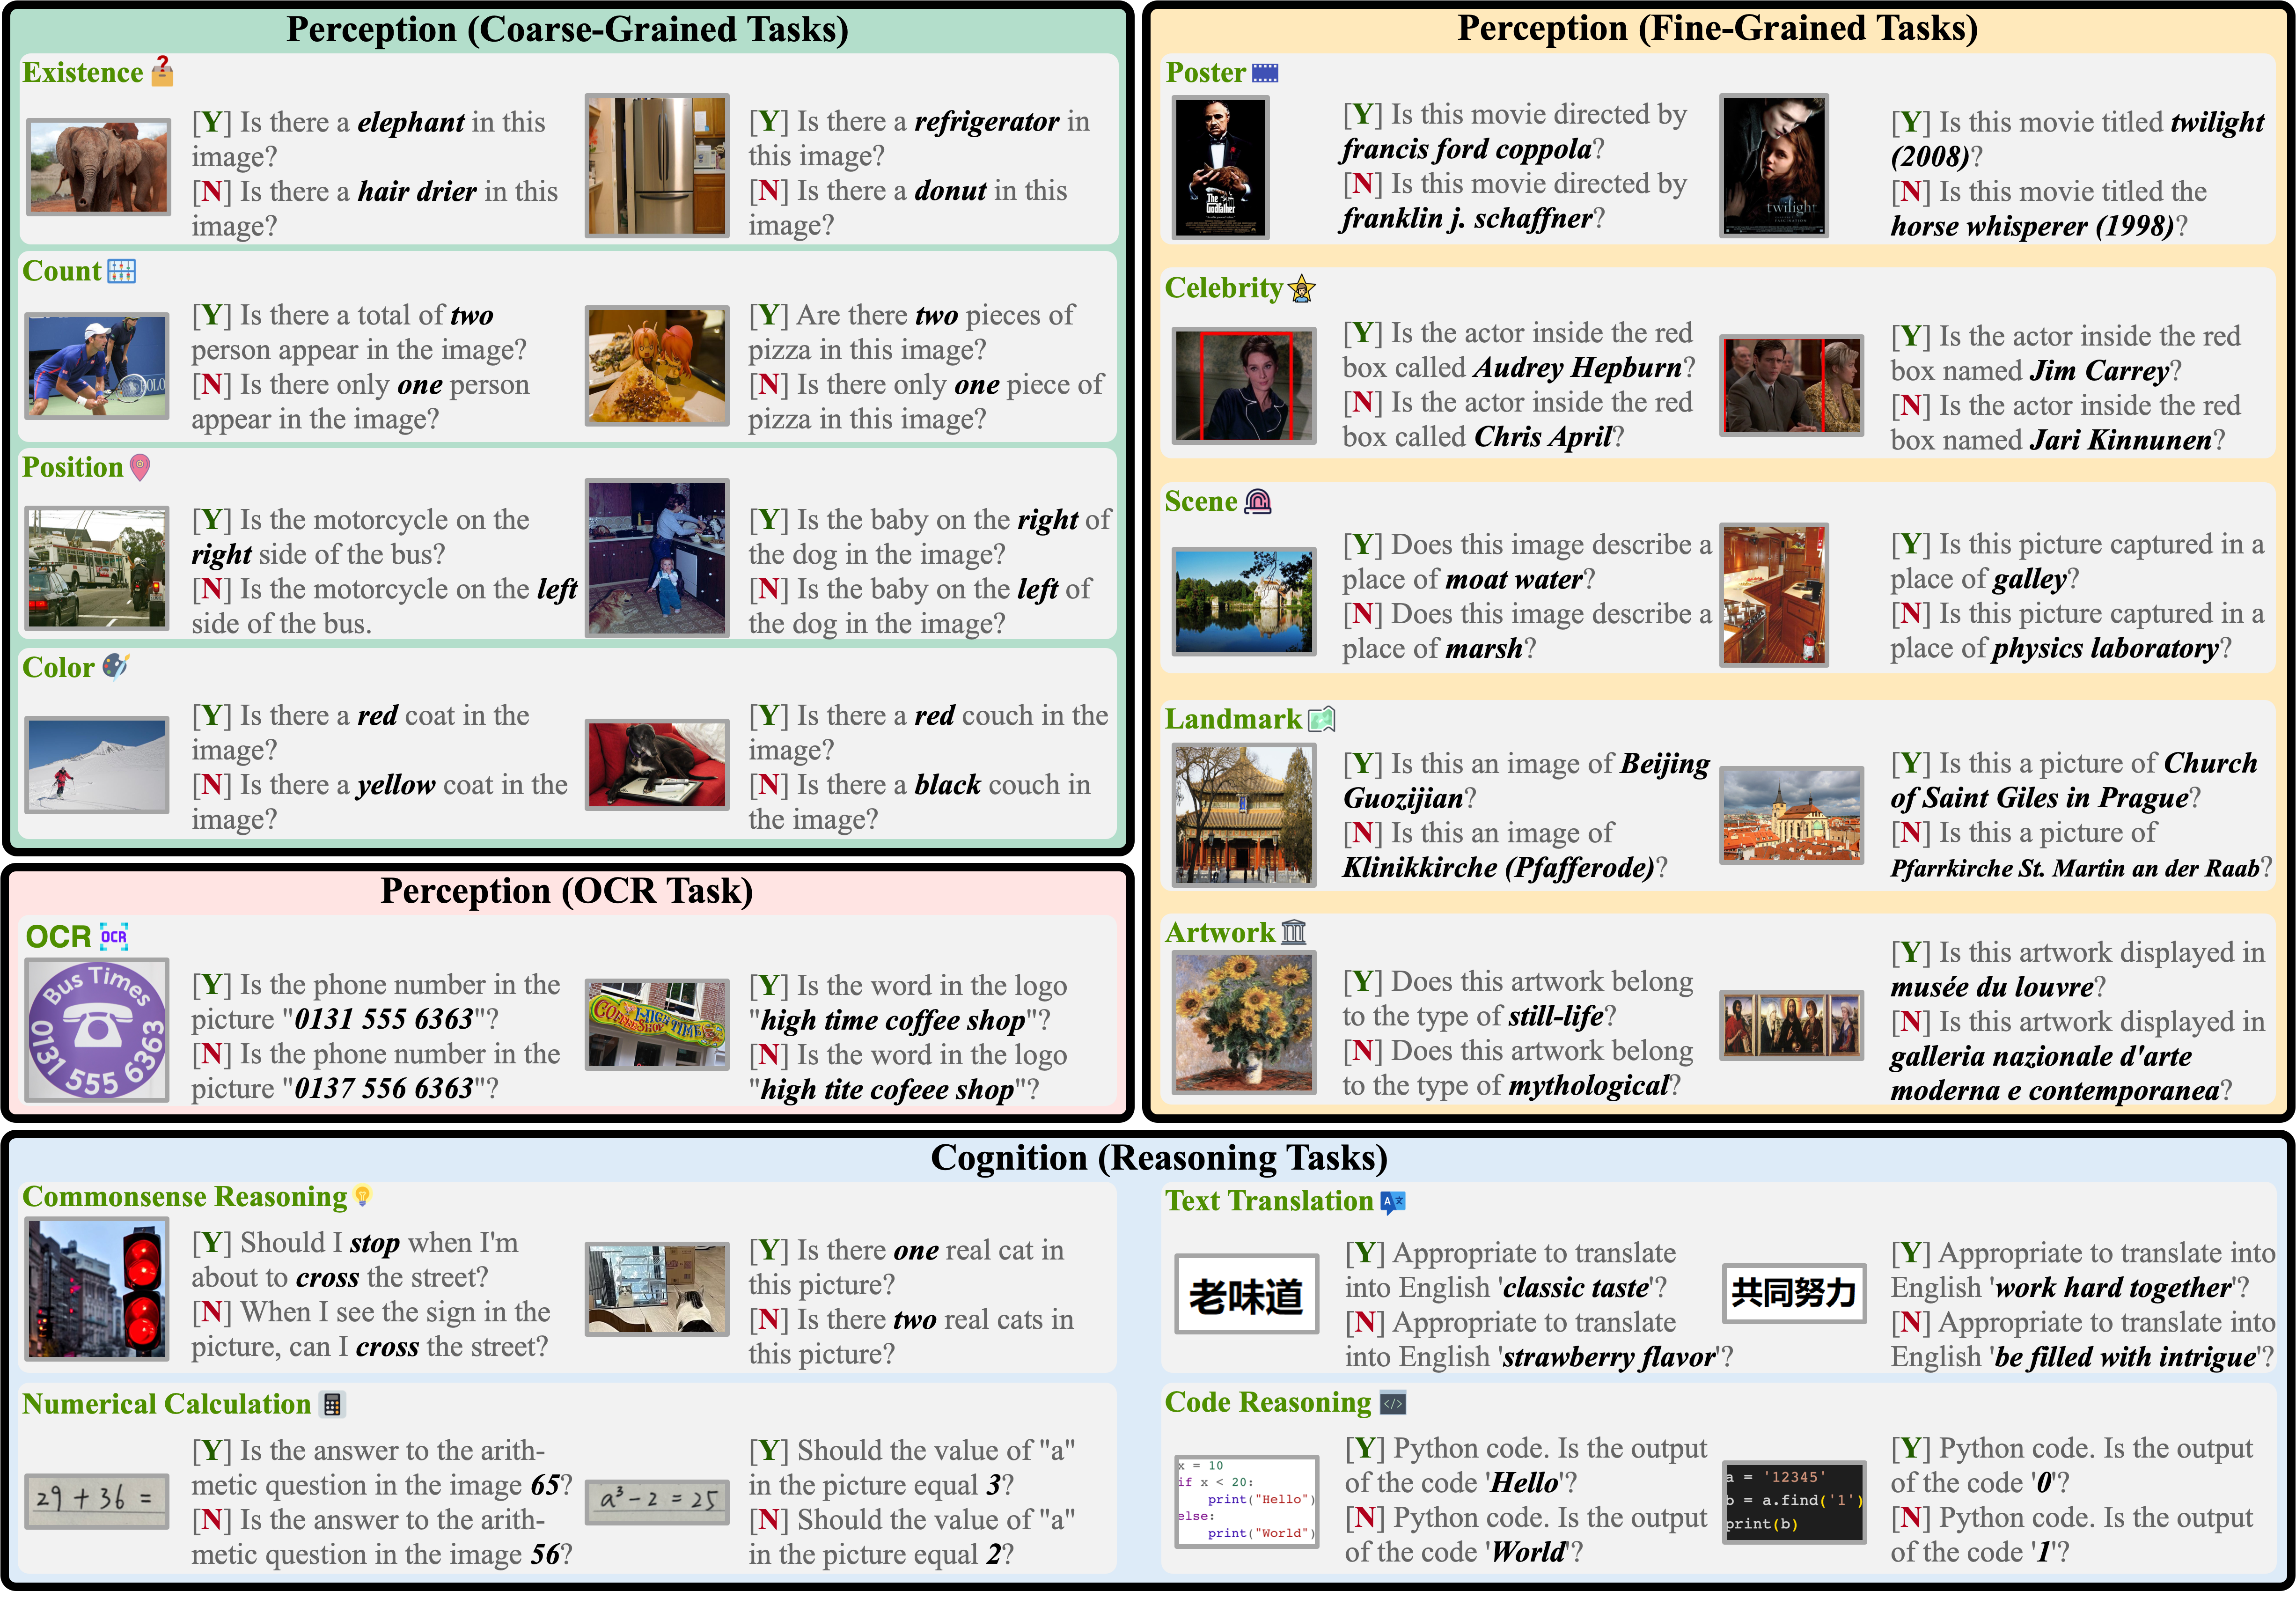
\includegraphics[height=6cm]{./p1.png}
\end{center}
\end{frame}

\begin{frame}[label={sec:orgb751986}]{Overview}
\begin{itemize}
\item \alert{Multimodal Instruction Tuning (M-IT)}
\item Multimodal In-Context Learning (M-ICL),
\item Multimodal Chain-of-Thought (M-CoT),
\item LLM-Aided Visual Reasoning (LAVR)
\end{itemize}
\end{frame}

\section{Multimodal Instruction Tuning (M-IT)}
\label{sec:org8bdfd34}

\begin{frame}[label={sec:orgcc40a04}]{Multimodal Instruction Tuning (M-IT)}
\begin{itemize}
\item Dataset:
\begin{itemize}
\item Existing benchmark datasets
\item Self-instruction
\end{itemize}
\item Model:
\begin{itemize}
\item Align foreign embeddings to the LLMs
\item Resort to expert models to translate foreign modalities into natural languages that LLMs can ingest
\end{itemize}
\item Fine-tuning:
\begin{itemize}
\item LoRA
\end{itemize}
\end{itemize}
\end{frame}

\begin{frame}[label={sec:orgbc4bd68}]{Multimodal Instruction Tuning (M-IT)}
\begin{itemize}
\item Works:
\begin{itemize}
\item MiniGPT-4\footfullcite{zhuMiniGPT4EnhancingVisionLanguage2023}
\item Visual Instruction Tuning (LLaVA) \footfullcite{liuVisualInstructionTuning2023}
\item mPLUG-Owl\footfullcite{yeMPLUGOwlModularizationEmpowers2023}
\end{itemize}
\end{itemize}
\end{frame}

\section{MiniGPT-4}
\label{sec:org372cd96}

\begin{frame}[label={sec:org21a5123}]{MiniGPT-4}
\begin{center}
\includegraphics[height=8cm]{./p2.png}
\end{center}
\end{frame}

\begin{frame}[label={sec:org7d67193}]{MiniGPT-4 methods}
\begin{itemize}
\item Vicuna (LLaMA)
\item BLIP-2 (ViT backbone with pre-trained Q-Former)
\item Linear projection to bridge the gap
\item Two stages
\begin{itemize}
\item Pretraining the model on a large collection of aligned image-text pairs to acquire visionlanguage knowledge.
\item Fine-tune the pretrained model with a smaller but high-quality image-text dataset with a designed conversational template to enhance the model’s generation reliability and usability.
\end{itemize}
\end{itemize}
\end{frame}

\begin{frame}[label={sec:org57fc3e0}]{MiniGPT-4 First stage}
\begin{itemize}
\item Train
\begin{itemize}
\item Conceptual Caption, SBU, and LAION
\item 20,000 training steps with a batch size of 256, covering approximately 5 million image-text pairs.
\end{itemize}
\item Issues
\begin{itemize}
\item Generating repetitive words or sentences, fragmented sentences, or irrelevant content.
\end{itemize}
\end{itemize}
\end{frame}

\begin{frame}[label={sec:org73dfd89},fragile]{MiniGPT-4 First stage alignment}
 \begin{itemize}
\item Two step
\begin{itemize}
\item Align the image-text pairs generation (Template)
\begin{itemize}
\item \texttt{\#\#\#Human: <Img><ImageFeature></Img> Describe this image in detail. Give as many details as possible. Say everything you see. \#\#\#Assistant:}
\end{itemize}
\item Data post processing (ChatGPT, fix the generated text)
\end{itemize}
\end{itemize}
\end{frame}

\begin{frame}[label={sec:org1e07214},fragile]{MiniGPT-4 Final fine-tuning}
 \begin{itemize}
\item Finetune the pretrained model with the curated high-quality image-text pairs.

\item \texttt{\#\#\#Human: <Img><ImageFeature></Img> <Instruction> \#\#\#Assistant:}
\end{itemize}
\end{frame}

\begin{frame}[label={sec:orgc5fa8ac}]{LLaVA}
\begin{center}
\includegraphics[width=.9\linewidth]{./p3.png}
\end{center}
\end{frame}

\section{Reference}
\label{sec:org76ee680}

\begin{frame}[allowframebreaks]{Reference}
\printbibliography
\end{frame}
\end{document}